% AA-05 | Algebra abstrakcyjna | Iteracja 03
\chapter[Szeregi podnormalne i nilpotentność]{Szeregi podnormalne, grupy rozwiązalne i nilpotentne}
\label{aa:ch:szeregi}

\section{Dlaczego rozkładamy grupę na czynniki?}
Klasyfikowanie grup wyłącznie na podstawie ich rzędu rzadko się udaje.
Możemy jednak badać grupę przez podgrupę normalną $N\trianglelefteq G$
i grupę ilorazową $G/N$. Proces ten przypomina rozkład liczby
na czynniki pierwsze, lecz czynniki grupowe mogą być nieprzemienne,
a ich kolejność i sposób ponownego składania mają znaczenie.
W tym rozdziale udowodnimy, w jakim sensie lista najprostszych czynników
jest niezależna od wybranego rozkładu; następnie rozróżnimy
\emph{rozwiązalność}, która kontroluje kolejne komutatory,
i silniejszą własność \emph{nilpotentności}.

\begin{definicja}[Grupa prosta]
\label{aa:def:prosta}
Grupę $G\ne\{e\}$ nazywamy \emph{prostą}, jeśli jedynymi
podgrupami normalnymi $G$ są $\{e\}$ i $G$.
Podgrupa $N\trianglelefteq G$ jest \emph{maksymalną właściwą podgrupą
normalną}, jeżeli $N\ne G$ oraz nie istnieje
$K\trianglelefteq G$ z $N\subsetneq K\subsetneq G$.
\end{definicja}
\begin{lemat}[Proste ilorazy]
\label{aa:lem:maxnormal}
Niech $N\trianglelefteq G$ będzie właściwą podgrupą normalną.
Wtedy $N$ jest maksymalna wśród właściwych podgrup normalnych $G$
dokładnie wtedy, gdy $G/N$ jest grupą prostą.
\end{lemat}
\begin{proof}
Twierdzenie o odpowiedniości podgrup
(\ref{aa:tw:odpowiedniosc}) daje bijekcję między podgrupami
$K$ takimi, że $N\subseteq K\le G$, a podgrupami $G/N$.
Ponadto $K$ jest normalna w $G$ dokładnie wtedy, gdy
$K/N$ jest normalna w $G/N$: równość
$(gN)(K/N)(gN)^{-1}=K/N$ oznacza $gKg^{-1}N=K$.
Ponieważ $gNg^{-1}=N\subseteq gKg^{-1}$, lewa strona
tej równości jest równa $gKg^{-1}$; otrzymujemy więc
warunek $gKg^{-1}=K$.
Zatem pośrednie właściwe podgrupy normalne są dokładnie
niebanalnymi właściwymi podgrupami normalnymi ilorazu.
Ich brak jest równoważny prostocie $G/N$.
\end{proof}

\begin{definicja}[Szereg podnormalny i kompozycyjny]
\label{aa:def:kompozycyjny}
Dla grupy $G$ \emph{szeregiem podnormalnym} nazywamy skończony ciąg
$G=G_0\trianglerighteq G_1\trianglerighteq\cdots\trianglerighteq G_r=\{e\}$,
w którym $G_{i+1}\trianglelefteq G_i$ dla każdego $i$.
Jego \emph{czynniki} to $G_i/G_{i+1}$.
Jeżeli wszystkie zawierania są właściwe, a każdy czynnik jest prosty,
mówimy o \emph{szeregu kompozycyjnym}.
Nie wymagamy, by $G_i$ były normalne w całej grupie $G$;
normalność dotyczy kolejnych sąsiadujących wyrazów.
\end{definicja}

\begin{twierdzenie}[Istnienie szeregu kompozycyjnego dla grup skończonych]
\label{aa:tw:existcomp}
Każda niebanalna grupa skończona $G$ posiada szereg kompozycyjny.
\end{twierdzenie}
\begin{proof}
Przeprowadzimy indukcję względem $|G|$.
Jeśli $G$ jest prosta, wystarcza $G\triangleright\{e\}$.
Jeśli nie jest prosta, zbiór właściwych podgrup normalnych
$G$ zawierających $\{e\}$ jest niepusty i skończony,
więc możemy wybrać podgrupę $N$ maksymalną względem zawierania.
Z poprzedniego lematu $G/N$ jest prosta.
Ponieważ $|N|<|G|$, założenie indukcyjne daje szereg
kompozycyjny $N=N_0\triangleright\cdots\triangleright N_s=\{e\}$
(gdy $N=\{e\}$, stosujemy szereg długości zero).
Dopisanie $G\triangleright N$ przed tym szeregiem daje
szereg kompozycyjny $G$, gdyż pierwszy czynnik $G/N$ jest prosty,
a wszystkie pozostałe czynniki pochodzą z szeregu $N$.
\end{proof}

\section{Twierdzenie Jordana--Höldera}
\begin{lemat}[Porównanie dwóch maksymalnych podgrup normalnych]
\label{aa:lem:two-max}
Niech $G$ będzie skończoną grupą, a $N,M$ dwiema różnymi
maksymalnymi właściwymi podgrupami normalnymi $G$.
Jeśli $L=N\cap M$, to $NM=G$,
$N/L\cong G/M$ oraz $M/L\cong G/N$.
W szczególności $N/L$ i $M/L$ są grupami prostymi.
\end{lemat}
\begin{proof}
Ponieważ $N$ i $M$ są normalne w $G$, zbiór
$NM=\{nm:n\in N,\ m\in M\}$ jest podgrupą normalną:
$(nm)(n'm')=n(mn'm^{-1})(mm')\in NM$.
Ponadto $(nm)^{-1}=m^{-1}n^{-1}
=(m^{-1}n^{-1}m)m^{-1}\in NM$, a $e\in NM$.
Sprzężenie przez dowolne $g\in G$ zachowuje oba czynniki,
zatem $NM$ jest podgrupą normalną $G$.
Gdyby $M\subseteq N$, maksymalność właściwej podgrupy normalnej
$M$ i normalność $N$ wymuszałyby $N=M$ albo $N=G$,
co przeczy założeniom. Zatem $NM$ zawiera właściwie $N$.
Z maksymalności $N$ dostajemy $NM=G$.

Rozważmy homomorfizm $f:N\to G/M$ dany wzorem $f(n)=nM$.
Jest surjektywny: każdy $g\in G=NM$ ma postać $nm$,
a wtedy $gM=nM$. Jądro to $N\cap M=L$.
Pierwsze twierdzenie o izomorfizmie daje $N/L\cong G/M$.
W ten sam sposób $M/L\cong G/N$.
Oba ilorazy po prawej są proste na mocy
Lematu~\ref{aa:lem:maxnormal}, więc również ilorazy po lewej.
\end{proof}

\begin{twierdzenie}[Jordana--Höldera]
\label{aa:tw:jordan-holder}
Niech $G$ będzie grupą skończoną. Jeśli
$G=G_0\triangleright G_1\triangleright\cdots\triangleright G_r=\{e\}$
oraz $G=H_0\triangleright H_1\triangleright\cdots\triangleright H_s=\{e\}$
są dwoma szeregami kompozycyjnymi, to $r=s$ i istnieje
permutacja $\sigma$ zbioru $\{0,\ldots,r-1\}$ taka, że
$G_i/G_{i+1}\cong H_{\sigma(i)}/H_{\sigma(i)+1}$
dla wszystkich $i$.
Nie twierdzimy, że czynniki w obu szeregach występują w tej samej kolejności.
\end{twierdzenie}
\begin{proof}
Przeprowadzimy indukcję względem $|G|$. Dla grupy trywialnej
oba szeregi mają długość zero. Dla grupy prostej każdy szereg
kompozycyjny ma długość jeden i tezę widać bezpośrednio.
Niech teraz $G$ będzie nieprosta i niech $N=G_1$, $M=H_1$.
Podgrupy $N,M$ są maksymalnymi właściwymi podgrupami normalnymi
$G$, bo $G/N$ i $G/M$ są proste.

Jeśli $N=M$, początkowe czynniki $G/N$ i $G/M$ są jednakowe,
a pozostałe części obu szeregów są szeregami kompozycyjnymi $N$.
Ponieważ $|N|<|G|$, założenie indukcyjne utożsamia ich
czynniki z dokładnością do permutacji. Dołączając wspólny czynnik
$G/N$, otrzymujemy tezę.

Niech $N\ne M$ i $L=N\cap M$.
Poprzedni lemat daje proste ilorazy
$N/L\cong G/M$ oraz $M/L\cong G/N$.
Wybierzmy szereg kompozycyjny $L$: jeśli $L=\{e\}$,
przyjmujemy szereg długości zero, a jeśli $L\ne\{e\}$,
jego istnienie zapewnia Twierdzenie~\ref{aa:tw:existcomp}.
Oznaczmy wielozbiór \emph{typów izomorfizmu} jego czynników
przez $\mathcal F(L)$. Zapis $\{\!\{Q_1,\ldots,Q_k\}\!\}$ oznacza wielozbiór
z zachowaniem krotności, a $\uplus$ oznacza sumę takich wielozbiorów.
Dopisanie $N\triangleright L$ do tego szeregu daje szereg
kompozycyjny $N$, którego lista czynników składa się
z $N/L$ i czynników $\mathcal F(L)$.
Ponieważ $|N|<|G|$, założenie indukcyjne zastosowane do dwóch
szeregów kompozycyjnych $N$ (oryginalnego ogona
$G_1\triangleright\cdots\triangleright G_r$
i właśnie skonstruowanego) pokazuje, że czynniki oryginalnego
ogona są, z dokładnością do permutacji, równe
$\{\!\{N/L\}\!\}\uplus\mathcal F(L)$.
Analogiczne rozumowanie dla $M$ daje
$\{\!\{M/L\}\!\}\uplus\mathcal F(L)$.

Dołączamy pierwsze czynniki $G/N$ i $G/M$.
Dla pierwszego szeregu dostajemy wielozbiór
$\{\!\{G/N,\ N/L\}\!\}\uplus\mathcal F(L)$,
a dla drugiego
$\{\!\{G/M,\ M/L\}\!\}\uplus\mathcal F(L)$.
Izomorfizmy z poprzedniego lematu zamieniają parami
$G/N\cong M/L$ i $G/M\cong N/L$, więc oba wielozbiory
są takie same z dokładnością do izomorfizmu. Ich liczności
są zatem równe, co daje również $r=s$.
\end{proof}

\begin{lemat}[Proste grupy abelowe skończone]
\label{aa:lem:finite-abelian-simple}
Niech $G$ będzie niebanalną skończoną grupą abelową.
Wtedy $G$ jest grupą prostą dokładnie wtedy, gdy
$G\cong C_p$ dla pewnej liczby pierwszej $p$.
\end{lemat}
\begin{proof}
Załóżmy, że $G$ jest prosta. Wybierzmy element $g\ne e$.
Podgrupa $\langle g\rangle$ jest niebanalna. Każda podgrupa
grupy abelowej jest normalna, zatem prostota $G$ wymusza
$\langle g\rangle=G$: grupa $G$ jest cykliczna.
Niech $n=|G|$ będzie rzędem jej generatora.
Gdyby $n$ było liczbą złożoną, istniałby dzielnik $d$
spełniający $1<d<n$. Element $g^{n/d}$ miałby rząd $d$:
$(g^{n/d})^d=e$, a dla $0<k<d$ nierówność
$0<kn/d<n$ wyklucza $(g^{n/d})^k=e$.
Wówczas $\langle g^{n/d}\rangle$ byłaby niebanalną,
właściwą podgrupą normalną $G$, co jest sprzeczne
z prostotą. Zatem $n=p$ jest liczbą pierwszą.

Odwrotnie, w grupie cyklicznej $C_p$ rzędu pierwszego
rząd każdej podgrupy dzieli $p$ na mocy twierdzenia Lagrange'a.
Może więc wynosić tylko $1$ albo $p$, a zatem
$C_p$ nie ma niebanalnych właściwych podgrup normalnych.
\end{proof}

\begin{przyklad}[Ta sama lista czynników, inna kolejność]
\label{aa:prz:jordan-c6}
Rozważmy addytywną grupę $C_6=\mathbb Z/6\mathbb Z$.
Ma ona podgrupy $H_2=\{[0]_6,[3]_6\}$ rzędu $2$
oraz $H_3=\{[0]_6,[2]_6,[4]_6\}$ rzędu $3$.
W grupie abelowej obie są normalne. Istnieją zatem
różne szeregi kompozycyjne
\[
 C_6\triangleright H_2\triangleright\{0\},\qquad
 C_6\triangleright H_3\triangleright\{0\}.
\]
Pierwszy ma czynniki $C_6/H_2\cong C_3$ i
$H_2\cong C_2$, drugi zaś $C_6/H_3\cong C_2$ i
$H_3\cong C_3$. Izomorfizm ilorazu z $C_3$
w pierwszym szeregu jest indukowany przez redukcję
klas modulo $3$; analogicznie redukcja modulo $2$
opisuje drugi. Czynniki występują w innej kolejności,
lecz ich wielozbiór z dokładnością do izomorfizmu
pozostaje niezmieniony, jak przewiduje
Twierdzenie~\ref{aa:tw:jordan-holder}.
\end{przyklad}

\begin{figure}[htbp]
\centering
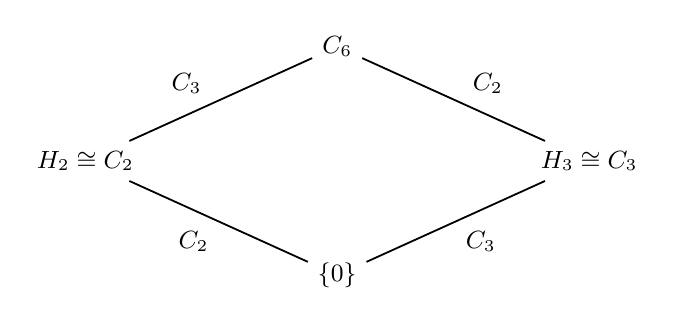
\begin{tikzpicture}[every node/.style={font=\small},line width=.65pt]
 \node (G) at (0,2.8) {$C_6$};
 \node (H2) at (-3.2,1.35) {$H_2\cong C_2$};
 \node (H3) at (3.2,1.35) {$H_3\cong C_3$};
 \node (E) at (0,-.1) {$\{0\}$};
 \draw (G) -- node[above left,pos=.55] {$C_3$} (H2);
 \draw (G) -- node[above right,pos=.55] {$C_2$} (H3);
 \draw (H2) -- node[below left,pos=.5] {$C_2$} (E);
 \draw (H3) -- node[below right,pos=.5] {$C_3$} (E);
\end{tikzpicture}
\caption{Dwie różne drogi od $C_6$ do podgrupy trywialnej.
 Etykieta każdej krawędzi oznacza izomorficzny typ odpowiedniego
 ilorazu. Obie drogi mają czynniki $C_2$ i $C_3$, ale w odwrotnej
 kolejności.}
\label{aa:fig:c6-composition-chains}
\end{figure}

\begin{przyklad}[Szereg kompozycyjny $S_3$ i kolejność czynników]
\label{aa:prz:jordan-s3}
Oznaczmy przez $A_3=\langle(1\,2\,3)\rangle$ podgrupę
rzędu $3$ grupy $S_3$. Szereg
$S_3\triangleright A_3\triangleright\{e\}$
ma czynniki $S_3/A_3\cong C_2$ oraz $A_3\cong C_3$.
Nie możemy zacząć od żadnej podgrupy rzędu $2$,
ponieważ nie jest ona normalna w $S_3$.
To przykład, w którym kolejność czynników jest wymuszona przez strukturę grupy.
\end{przyklad}

\begin{przyklad}[Szereg w $A_4$ i subtelność normalności]
\label{aa:prz:jordan-a4}
Niech $V_4=\{e,a,b,c\}$, gdzie
$a=(1\,2)(3\,4)$, $b=(1\,3)(2\,4)$,
$c=(1\,4)(2\,3)$.
Jest to normalna podgrupa $A_4$ rzędu $4$
(Przykład~\ref{aa:prz:sylow-a4}).
Wybierzmy $K=\{e,(1\,2)(3\,4)\}$.
Ponieważ $V_4$ jest abelowa, $K\trianglelefteq V_4$.
Zatem
$A_4\triangleright V_4\triangleright K\triangleright\{e\}$
jest szeregiem kompozycyjnym o czynnikach
$C_3,C_2,C_2$ (w tej kolejności).
Jednak $K$ nie jest normalna w $A_4$: sprzężenie
przez $(1\,2\,3)$ przekształca $(1\,2)(3\,4)$
w $(1\,4)(2\,3)$, co nie należy do $K$.
Właśnie dlatego definicja szeregu wymaga normalności
w wyrazie poprzednim, a nie w całym $G$.
\end{przyklad}

\begin{uwaga}[Czego twierdzenie nie mówi?]
Czynniki kompozycyjne nie wyznaczają grupy z dokładnością do
izomorfizmu. Na przykład $C_4$ oraz $C_2\times C_2$
mają po dwa czynniki kompozycyjne izomorficzne z $C_2$,
a jednak nie są izomorficzne: pierwsza grupa ma element
rzędu $4$, druga nie. W kolejnym rozdziale zobaczymy,
że sposób składania grup z tych samych czynników jest
odrębną informacją, opisywaną przez rozszerzenia grup.
\end{uwaga}

\section{Komutatory i grupy rozwiązalne}
\begin{definicja}[Komutator i podgrupa pochodna]
\label{aa:def:pochodna}
Dla $x,y\in G$ kładziemy $[x,y]=xyx^{-1}y^{-1}$.
Dla podgrup $A,B\le G$ oznaczamy przez $[A,B]$ podgrupę
wygenerowaną przez wszystkie $[a,b]$, gdzie $a\in A$, $b\in B$.
\emph{Podgrupą pochodną} $G'=[G,G]$ nazywamy podgrupę
generowaną przez wszystkie komutatory elementów $G$.
\end{definicja}
\begin{lemat}[Najmniejsza normalna podgrupa o abelowym ilorazie]
\label{aa:lem:derived-abelian}
Dla każdej grupy $G$ podgrupa $G'$ jest charakterystyczna
(to znaczy: zachowuje ją każdy automorfizm $G$),
a więc normalna w $G$. Iloraz $G/G'$ jest abelowy.
Jeżeli $N\trianglelefteq G$, to $G/N$ jest abelowa
dokładnie wtedy, gdy $G'\subseteq N$.
\end{lemat}
\begin{proof}
Każdy automorfizm $\alpha:G\to G$ spełnia
$\alpha([x,y])=[\alpha(x),\alpha(y)]$, zatem
przekształca zbiór wszystkich komutatorów na ten sam zbiór.
Dlatego $\alpha(G')=G'$, co jest charakterystycznością.
Każde sprzężenie jest automorfizmem, więc $G'\trianglelefteq G$.
W ilorazie $G/G'$ równość $[x,y]\in G'$ daje
$(xG')(yG')=(yG')(xG')$, czyli przemienność.
Dla ogólnej $N\trianglelefteq G$ analogicznie:
$G/N$ jest abelowa wtedy i tylko wtedy, gdy
$(xyx^{-1}y^{-1})N=N$ dla wszystkich $x,y$,
czyli gdy wszystkie komutatory, a więc $G'$, należą do $N$.
\end{proof}

\begin{definicja}[Szereg pochodny i rozwiązalność]
\label{aa:def:rozwiazalna}
Definiujemy $G^{(0)}=G$ oraz $G^{(i+1)}=[G^{(i)},G^{(i)}]$
dla $i\ge0$. Jest to \emph{szereg pochodny} $G$.
Grupa $G$ jest \emph{rozwiązalna}, jeśli istnieje $r\ge0$
z $G^{(r)}=\{e\}$.
Najmniejsze takie $r$ nazywamy jej długością pochodną.
\end{definicja}

\begin{twierdzenie}[Kryterium rozwiązalności przez ilorazy abelowe]
\label{aa:tw:solvable-series}
Grupa $G$ jest rozwiązalna wtedy i tylko wtedy, gdy istnieje
skończony szereg podnormalny
$G=G_0\trianglerighteq G_1\trianglerighteq\cdots
\trianglerighteq G_r=\{e\}$,
w którym każdy iloraz $G_i/G_{i+1}$ jest abelowy.
\end{twierdzenie}
\begin{proof}
Jeśli $G^{(r)}=\{e\}$, szereg pochodny od $G^{(0)}$
do $G^{(r)}$ jest żądanym szeregiem:
$G^{(i+1)}$ jest normalna w $G^{(i)}$,
a $G^{(i)}/G^{(i+1)}$ jest abelowy
z poprzedniego lematu.

Odwrotnie, niech dany będzie szereg o abelowych czynnikach.
Pokażemy indukcyjnie $G^{(i)}\subseteq G_i$.
Dla $i=0$ jest to równość. Gdy $G^{(i)}\subseteq G_i$,
to
$G^{(i+1)}=[G^{(i)},G^{(i)}]\subseteq[G_i,G_i]$.
Ponieważ $G_i/G_{i+1}$ jest abelowy,
Lemat~\ref{aa:lem:derived-abelian} zastosowany do $G_i$
daje $[G_i,G_i]\subseteq G_{i+1}$.
Otrzymujemy więc $G^{(i+1)}\subseteq G_{i+1}$.
Dla $i=r$ mamy $G^{(r)}\subseteq G_r=\{e\}$,
co kończy dowód.
\end{proof}

\begin{lemat}[Podgrupy, ilorazy i rozszerzenia grup rozwiązalnych]
\label{aa:lem:solvable-extension}
Niech $G$ będzie grupą, $H\le G$ i $N\trianglelefteq G$.
\begin{enumerate}
\item Jeśli $G$ jest rozwiązalna, to $H$ i $G/N$ są rozwiązalne.
\item Jeśli $N$ i $G/N$ są rozwiązalne, to $G$ jest rozwiązalna.
\end{enumerate}
\end{lemat}
\begin{proof}
Dla podgrupy $H$ indukcja daje
$H^{(i)}\subseteq G^{(i)}$, bo komutatory elementów
$H^{(i)}$ są komutatorami elementów $G^{(i)}$.
Jeśli więc $G^{(r)}=\{e\}$, także $H^{(r)}=\{e\}$.
Niech $\pi:G\to G/N$ będzie naturalnym rzutem.
Dla każdego $i$ mamy
$\pi(G^{(i)})=(G/N)^{(i)}$:
w bazie $i=0$ jest to surjektywność $\pi$, a krok indukcyjny
wynika z $\pi([x,y])=[\pi(x),\pi(y)]$ i zachowania
generowania podgrupy przez homomorfizm.
Jeśli $G^{(r)}=\{e\}$, to $(G/N)^{(r)}=\{e\}$.

Załóżmy teraz $N^{(s)}=\{e\}$ i $(G/N)^{(r)}=\{e\}$.
Powyższa równość obrazów oznacza $G^{(r)}\subseteq N$.
Dla dowolnej podgrupy $A\le B$ zachodzi $A^{(j)}\subseteq B^{(j)}$,
zatem $(G^{(r)})^{(s)}\subseteq N^{(s)}=\{e\}$.
Z definicji szeregu pochodnego
$(G^{(r)})^{(s)}=G^{(r+s)}$, co dowodzi rozwiązalności $G$.
\end{proof}

\begin{twierdzenie}[Czynniki kompozycyjne a rozwiązalność]
\label{aa:tw:solvable-composition-factors}
Niech $G$ będzie grupą skończoną. Następujące warunki są
równoważne:
\begin{enumerate}
\item $G$ jest rozwiązalna;
\item w każdym szeregu kompozycyjnym $G$ wszystkie czynniki
są cykliczne o rzędach pierwszych;
\item istnieje szereg kompozycyjny $G$, w którym wszystkie
czynniki są cykliczne o rzędach pierwszych.
\end{enumerate}
Dla $G=\{e\}$ dwa ostatnie warunki rozumiemy jako prawdziwe:
pusty szereg nie ma czynników.
\end{twierdzenie}
\begin{proof}
Dla grupy trywialnej teza wynika bezpośrednio z definicji.
Niech $G$ będzie niebanalna; na mocy
Twierdzenia~\ref{aa:tw:existcomp} posiada szereg kompozycyjny.

Załóżmy (1) i wybierzmy dowolny szereg kompozycyjny
$G=G_0\triangleright\cdots\triangleright G_r=\{e\}$.
Z Lematu~\ref{aa:lem:solvable-extension} wynika, że
każda podgrupa $G_i$ jest rozwiązalna, a ponieważ
$G_{i+1}\trianglelefteq G_i$, również iloraz
$S_i=G_i/G_{i+1}$ jest rozwiązalny. Jest to grupa prosta.
Podgrupa pochodna $S_i'$ jest w $S_i$ normalna, zatem
$S_i'=\{e\}$ albo $S_i'=S_i$. Drugi przypadek
powodowałby $S_i^{(k)}=S_i\ne\{e\}$ dla każdego $k\ge1$,
co przeczy rozwiązalności. Wobec tego $S_i'=\{e\}$.
Z Lematu~\ref{aa:lem:derived-abelian} wynika, że
$S_i$ jest abelowa, a z
Lematu~\ref{aa:lem:finite-abelian-simple}, że $S_i\cong C_{p_i}$
dla pewnej liczby pierwszej $p_i$. Ponieważ wybrany szereg
był dowolny, otrzymaliśmy (2).

Implikacja (2)$\Rightarrow$(3) wynika z istnienia
szeregu kompozycyjnego. Przy (3) mamy szereg podnormalny
z abelowymi ilorazami, gdyż każda grupa $C_{p_i}$
jest abelowa. Twierdzenie~\ref{aa:tw:solvable-series}
daje rozwiązalność $G$, czyli (1).
\end{proof}

\begin{przyklad}[Grupy $S_3$, $S_4$ i $A_5$]
Dla $S_3$ podgrupa komutatorowa to $A_3$.
Zawieranie $S_3'\subseteq A_3$ wynika z abelowości
$S_3/A_3\cong C_2$. Ponadto $S_3$ nie jest abelowa,
więc $S_3'\ne\{e\}$. Ponieważ $A_3$ ma rząd pierwszy,
musi być $S_3'=A_3$; dalej $A_3'=\{e\}$.
Grupa $S_3$ jest zatem rozwiązalna o długości pochodnej $2$.
Grupa $S_4$ ma szereg normalności kolejnych wyrazów
$S_4\triangleright A_4\triangleright V_4\triangleright\{e\}$
o abelowych ilorazach $C_2,C_3,V_4$, więc jest rozwiązalna.
Możemy tu dokładniej wyznaczyć szereg pochodny.
Homomorfizm znaku pokazuje $S_4'\subseteq A_4$.
Komutator dwóch transpozycji o jednym wspólnym punkcie,
na przykład $[(1\,2),(2\,3)]$, jest $3$-cyklem.
Ponieważ $S_4'$ jest normalna w $S_4$, zawiera więc
wszystkie $3$-cykle, które są sprzężone w $S_4$.
Każdą parzystą permutację można zapisać jako iloczyn
parzystej liczby transpozycji, a następnie pogrupować je w pary.
Każdą taką parę zastępujemy iloczynem $3$-cykli:
parę jednakowych transpozycji usuwamy, parę różnych
transpozycji o jednym wspólnym punkcie zastępujemy
$3$-cyklem, a parę rozłączną, $(a\,b)(c\,d)$, zapisujemy
jako $(a\,c\,b)(a\,c\,d)$, przy przyjętym składaniu
od prawej do lewej. Zatem $S_4'=A_4$.

Dalej $A_4'\subseteq V_4$, gdyż $A_4/V_4\cong C_3$.
Jednak $A_4$ nie jest abelowa: $3$-cykle $(1\,2\,3)$
i $(1\,2\,4)$ nie komutują, zatem $A_4'\ne\{e\}$.
Podgrupa $A_4'$ jest normalna w $A_4$, więc wraz
z dowolnym niezerowym elementem $V_4$ zawiera jego
wszystkie sprzężenia w $A_4$. Trzy nieidentycznościowe
elementy $V_4$ są sprzężone przez $3$-cykle,
a więc $A_4'=V_4$. Ponieważ $V_4$ jest abelowa,
$V_4'=\{e\}$. Ostatecznie szereg pochodny ma postać
$S_4\triangleright A_4\triangleright V_4\triangleright\{e\}$,
a długość pochodna $S_4$ wynosi dokładnie $3$.
Dla $A_5$ sytuacja jest inna: pokażemy poniżej,
że to grupa prosta i nieabelowa, co wykluczy rozwiązalność.
\end{przyklad}

\section{Nieabelowa grupa prosta: \texorpdfstring{$A_5$}{A5}}
\begin{twierdzenie}[Prostota grupy alternującej $A_5$]
\label{aa:tw:a5-simple}
Grupa $A_5$, składająca się z parzystych permutacji pięciu punktów,
ma rząd $60$ i jest nieabelową grupą prostą.
\end{twierdzenie}
\begin{proof}
Mamy $|A_5|=5!/2=60$ na mocy homomorfizmu znaku
(\ref{aa:lem:znak}). Wypiszemy wszystkie klasy sprzężoności
w $A_5$, wyprowadzając ich rozmiary zamiast przyjmować je jako dane.
Elementami $A_5$ są: identyczność, $20$ cykli długości $3$,
$15$ iloczynów dwóch rozłącznych transpozycji i $24$ cykle długości $5$.
Rachunki są następujące: $\binom53\cdot2=20$,
$\binom54\cdot3=15$, a $5!/5=24$.
Nie ma innych typów parzystych permutacji pięciu punktów.

Rozważmy $c=(1\,2\,3)$. Permutacja $g\in S_5$ komutująca
z $c$ musi zachowywać nośnik $\{1,2,3\}$ i działać na nim
jak jedna z trzech potęg $c$; na dwóch pozostałych punktach
może wykonać dowolną permutację. Zatem $|C_{S_5}(c)|=3\cdot2=6$,
a dokładnie trzy takie permutacje są parzyste,
więc $|C_{A_5}(c)|=3$. Klasa $c$ w $A_5$ ma $60/3=20$
elementów; obejmuje zatem wszystkie cykle długości $3$.

Dla $d=(1\,2)(3\,4)$ element centralizatora w $S_5$
musi ustalać $5$ i permutować dwie dwuelementowe pary
$\{1,2\}$, $\{3,4\}$: może zamieniać punkty wewnątrz każdej
pary (cztery możliwości) i ewentualnie zamienić całe pary
(dwie możliwości). Mamy więc $|C_{S_5}(d)|=8$.
Wśród tych ośmiu permutacji dokładnie cztery są parzyste:
mnożenie przez nieparzystą transpozycję $(1\,2)$
przełącza parzystość i pozostaje w centralizatorze.
Stąd $|C_{A_5}(d)|=4$ i klasa ma $60/4=15$ elementów.
Zawiera zatem wszystkie iloczyny dwóch rozłącznych transpozycji.

Dla pięciocyklu $u=(1\,2\,3\,4\,5)$ permutacja komutująca
z $u$ jest wyznaczona przez obraz punktu $1$;
jego obraz może być jednym z pięciu punktów, a następne obrazy
są wymuszone przez równość $gu=ug$.
Centralizator w $S_5$ to $\langle u\rangle$ rzędu $5$.
Wszystkie potęgi $u$ są parzyste, więc
$|C_{A_5}(u)|=5$. Klasa w $A_5$ ma $60/5=12$ elementów.
Ponieważ pięciocykli jest $24$, tworzą dwie takie klasy.
Ostatecznie klasy sprzężoności $A_5$ mają rozmiary
$1,15,20,12,12$.

Jeśli $N\trianglelefteq A_5$, to $N$ jest sumą rozłącznych
klas sprzężoności i zawiera identyczność. Dlatego $|N|$
ma postać $1$ powiększonego o sumę pewnych liczb z listy
$15,20,12,12$. Wszystkie możliwe wartości to
$1,13,16,21,25,28,33,36,40,45,48,60$.
Z twierdzenia Lagrange'a $|N|$ musi dzielić $60$,
a z wypisanej listy jedynie $1$ i $60$ są dzielnikami $60$.
Stąd $N=\{e\}$ lub $N=A_5$, czyli $A_5$ jest prosta.
Jest nieabelowa: dla $u=(1\,2\,3)$ i $v=(1\,2\,4)$
mamy $uvu^{-1}=(2\,3\,4)\ne(1\,2\,4)=v$,
zatem $uv\ne vu$.
\end{proof}

\begin{wniosek}[Dlaczego $A_5$ nie jest rozwiązalna?]
\label{aa:wn:a5-not-solvable}
Grupa $A_5$ nie jest rozwiązalna.
\end{wniosek}
\begin{proof}
Gdyby $(A_5)'=\{e\}$, grupa byłaby abelowa.
Skoro jest nieabelowa, $(A_5)'\ne\{e\}$.
Podgrupa pochodna jest normalna, a $A_5$ jest prosta,
więc $(A_5)'=A_5$. Indukcja daje $(A_5)^{(i)}=A_5$
dla wszystkich $i$, zatem szereg pochodny nigdy nie osiąga
podgrupy trywialnej.
\end{proof}

\section{Grupy nilpotentne i szeregi centralne}
\begin{definicja}[Dolny szereg centralny]
\label{aa:def:dolny-centralny}
Dla grupy $G$ definiujemy
$\gamma_1(G)=G$ i $\gamma_{i+1}(G)=[\gamma_i(G),G]$ dla $i\ge1$.
Grupa $G$ jest \emph{nilpotentna}, jeśli $\gamma_{c+1}(G)=\{e\}$
dla pewnej liczby całkowitej $c\ge0$.
Najmniejszą taką liczbę $c$ nazywamy \emph{klasą nilpotentności}.
Dla grupy trywialnej klasa wynosi $0$; dla niebanalnej grupy
abelowej wynosi $1$.
\end{definicja}
\begin{lemat}[Własności dolnego szeregu centralnego]
\label{aa:lem:lower-properties}
Dla dowolnej grupy $G$ wszystkie podgrupy $\gamma_i(G)$
są charakterystyczne w $G$ i tworzą ciąg malejący.
Jeżeli $c\ge1$, $\gamma_{c+1}(G)=\{e\}$ i
$\gamma_c(G)\ne\{e\}$, to $\gamma_c(G)\subseteq Z(G)$.
Ponadto każda grupa nilpotentna jest rozwiązalna.
\end{lemat}
\begin{proof}
Indukcyjnie załóżmy, że $\gamma_i(G)$ jest charakterystyczna.
Każdy automorfizm przenosi zbiór komutatorów
$[\gamma_i(G),G]$ na siebie, zatem
$\gamma_{i+1}(G)$ jest charakterystyczna.
Ponieważ $\gamma_1(G)=G$, dowodzi to pierwszej części.
Dla $i=1$ mamy $\gamma_2(G)\subseteq G=\gamma_1(G)$.
Gdy $\gamma_i(G)\subseteq\gamma_{i-1}(G)$,
każdy generator $[x,g]$, $x\in\gamma_i(G)$, należy również
 do $[\gamma_{i-1}(G),G]$, więc
$\gamma_{i+1}(G)\subseteq\gamma_i(G)$.
Jeśli $\gamma_{c+1}(G)=[\gamma_c(G),G]=\{e\}$,
to każdy element $\gamma_c(G)$ komutuje z każdym elementem $G$;
stąd $\gamma_c(G)\subseteq Z(G)$.

Dla rozwiązalności zauważmy, że $G^{(0)}=\gamma_1(G)$.
Gdy $G^{(i)}\subseteq\gamma_{i+1}(G)$, mamy
$G^{(i+1)}=[G^{(i)},G^{(i)}]
\subseteq[\gamma_{i+1}(G),\gamma_{i+1}(G)]
\subseteq[\gamma_{i+1}(G),G]=\gamma_{i+2}(G)$.
Tak więc $G^{(i)}\subseteq\gamma_{i+1}(G)$ dla wszystkich $i$.
W szczególności $G^{(c)}=\{e\}$, gdy $G$ jest nilpotentna
klasy $c$.
\end{proof}

\begin{definicja}[Górny szereg centralny]
\label{aa:def:gorny-centralny}
Definiujemy $Z_0(G)=\{e\}$, a następnie rekurencyjnie
$Z_{i+1}(G)$ jako pełny przeciwobraz centrum grupy $G/Z_i(G)$
w naturalnym rzucie $G\to G/Z_i(G)$.
Zatem $Z_{i+1}(G)/Z_i(G)=Z(G/Z_i(G))$.
Konstrukcja jest poprawnie określona: $Z_0(G)$ jest normalna,
a jeśli $Z_i(G)\trianglelefteq G$, to przeciwobraz centrum
ilorazu jest również normalny w $G$.
W szczególności $Z_1(G)=Z(G)$.
\end{definicja}
\begin{lemat}[Porównanie dolnego i górnego szeregu centralnego]
\label{aa:lem:upper-lower}
Dla grupy $G$ i liczby całkowitej $c\ge0$ następujące warunki
są równoważne: (i) $\gamma_{c+1}(G)=\{e\}$;
(ii) $Z_c(G)=G$.
\end{lemat}
\begin{proof}
Najpierw wyjaśnijmy, że dla dowolnej podgrupy normalnej
$K\trianglelefteq G$ jej przeciwobraz centrum ilorazu
$G/K$ składa się dokładnie z tych $g\in G$, dla których
$[g,x]\in K$ dla każdego $x\in G$.
Wynika to bezpośrednio z równości
$[gK,xK]=[g,x]K$.

Załóżmy $Z_c(G)=G$. Dowodzimy przez indukcję po $j$, że
$\gamma_{j+1}(G)\subseteq Z_{c-j}(G)$ dla $0\le j\le c$.
Dla $j=0$ jest to $G\subseteq Z_c(G)$.
Jeśli $j<c$ i $\gamma_{j+1}(G)\subseteq Z_{c-j}(G)$,
to każdy komutator z elementem tej podgrupy i z $G$
należy do $Z_{c-j-1}(G)$, ponieważ
$[Z_{k+1}(G),G]\subseteq Z_k(G)$.
Stąd $\gamma_{j+2}(G)\subseteq Z_{c-j-1}(G)$.
W przypadku $j=c$ otrzymujemy $\gamma_{c+1}(G)\subseteq Z_0(G)=\{e\}$.

W drugą stronę załóżmy $\gamma_{c+1}(G)=\{e\}$.
Pokażemy indukcyjnie dla $0\le j\le c$ zawierania
$\gamma_{c-j+1}(G)\subseteq Z_j(G)$.
Dla $j=0$ jest to założenie. Jeśli $j<c$ i
$\gamma_{c-j+1}(G)\subseteq Z_j(G)$,
to $[\gamma_{c-j}(G),G]=\gamma_{c-j+1}(G)\subseteq Z_j(G)$.
Z podanego na początku opisu przeciwobrazu centrum
wynika $\gamma_{c-j}(G)\subseteq Z_{j+1}(G)$.
Dla $j=c$ dostajemy $\gamma_1(G)=G\subseteq Z_c(G)$,
więc $Z_c(G)=G$.
\end{proof}

\begin{twierdzenie}[Każda skończona $p$-grupa jest nilpotentna]
\label{aa:tw:pgroup-nilpotent}
Niech $G$ będzie skończoną grupą rzędu $p^a$, gdzie $p$
jest liczbą pierwszą, a $a\ge0$. Wtedy $G$ jest nilpotentna.
\end{twierdzenie}
\begin{proof}
Dla $a=0$ mamy $G=\{e\}$, a zatem już
$\gamma_1(G)=\{e\}$; grupa ta jest nilpotentna klasy $0$.
Niech $a\ge1$. Rozważmy górny szereg centralny.
Jeśli $Z_i(G)\ne G$, iloraz $G/Z_i(G)$ jest niebanalną
skończoną $p$-grupą. Z Twierdzenia~\ref{aa:tw:centrum-pgrupy}
jego centrum jest nietrywialne. Z definicji $Z_{i+1}(G)$
pełny przeciwobraz tego centrum zawiera właściwie $Z_i(G)$.
Wzrastający ciąg podgrup nie może mieć więcej niż $a$
ścisłych zawierań, ponieważ przy każdym ścisłym zawieraniu
rząd podgrupy rośnie co najmniej $p$ razy, a $|G|=p^a$.
Zatem po skończenie wielu krokach $Z_c(G)=G$.
Lemat~\ref{aa:lem:upper-lower} daje nilpotentność $G$.
\end{proof}

\begin{przyklad}[Grupa diedralna rzędu osiem]
\label{aa:prz:d8-nilpotent}
Niech $D_8=\langle r,s\mid r^4=e,\ s^2=e,\ srs=r^{-1}\rangle$
będzie grupą symetrii kwadratu, opisaną przez obrót o $90^\circ$
i odbicie (por. Przykład~\ref{aa:prz:d4}).
Zbiór jej elementów ma postać
$\{e,r,r^2,r^3,s,rs,r^2s,r^3s\}$.
Widać, że $[r,s]=rsr^{-1}s^{-1}=r^2$;
ponieważ $r^2$ komutuje z $r$ i $s$, jest centralny.
Iloraz przez $\langle r^2\rangle$ jest generowany przez
komutujące elementy rzędu $2$, więc jest abelowy.
Wobec tego $D_8'=\langle r^2\rangle$,
a $\gamma_3(D_8)=[\langle r^2\rangle,D_8]=\{e\}$.
Grupa $D_8$ jest nilpotentna klasy dokładnie $2$, lecz nie jest abelowa.
\end{przyklad}

\begin{przyklad}[Grupa rozwiązalna, która nie jest nilpotentna]
\label{aa:prz:s3-notnil}
Grupa $S_3$ jest rozwiązalna, jak dowiedliśmy powyżej,
lecz $Z(S_3)=\{e\}$: żaden nieidentycznościowy
$3$-cykl nie komutuje z transpozycją, a każda transpozycja
nie komutuje z inną transpozycją.
Gdyby $S_3$ była nilpotentna, ostatni nietrywialny wyraz
jej dolnego szeregu centralnego byłby, na mocy
Lematu~\ref{aa:lem:lower-properties}, zawarty w centrum.
Centrum jest jednak trywialne; sprzeczność.

Można też prześledzić dokładnie dolny szereg centralny.
Niech $r=(1\,2\,3)$ i $s=(1\,2)$.
Wtedy $srs^{-1}=r^{-1}$, a więc
$[r,s]=rsr^{-1}s^{-1}=r^2$.
W szczególności $[A_3,S_3]$ zawiera generator $r^2$
grupy $A_3$. Z drugiej strony
$[A_3,S_3]\subseteq A_3$, ponieważ $A_3$ jest normalna.
Zatem $[A_3,S_3]=A_3$. Wiemy już, że
$\gamma_2(S_3)=S_3'=A_3$, toteż rekurencyjnie
$\gamma_i(S_3)=A_3$ dla wszystkich $i\ge2$.
Szereg dolny nie osiąga zatem grupy trywialnej.
Rozwiązalność nie implikuje nilpotentności.
\end{przyklad}

\enlargethispage{3\baselineskip}
\begin{uwaga}[Co zostanie użyte przy konstrukcjach grup?]
W następnym rozdziale zobaczymy, jak z dwóch grup budować
iloczyny proste i półproste oraz jak interpretować rozszczepiające
się krótkie ciągi dokładne. Wykorzystamy te konstrukcje
do klasyfikacji grup rzędu $pq$ i do charakterystyki
skończonych grup nilpotentnych przez ich podgrupy Sylowa.
\end{uwaga}
